% +--------------------------------------------------------------------+
% | Sample Chapter 2
% +--------------------------------------------------------------------+

\cleardoublepage

% +--------------------------------------------------------------------+
% | Replace "This is Chapter 2" below with the title of your chapter.
% | LaTeX will automatically number the chapters.
% +--------------------------------------------------------------------+

\chapter{Bluetooth Low Energy}
\label{makereference2}

Bluetooth Low Energy (BLE, también denominado Bluetooth Smart) empezó como parte de la Bluetooth 4.0 Core Specification. Diseñado originalmente por Nokia bajo el nombre de Wibree, fue luego adoptado por el Bluetooth Special Interest Group (SIG).

El objetivo de Bluetooth Low Energy es complementar al Bluetooth clásico y ser la tecnología inalámbrica con el menor consumo energético posible. También tiene como objetivo producirse en grandes cantidades, para llegar a objetos que hasta ahora no disponían de ninguna conectividad inalámbrica. Para lograr estas grandes cantidades, se necesita tener un coste muy bajo, lo cual se consigue con tres elementos clave:

\begin{itemize}

	\item \textbf{Banda ISM:} BLE utiliza la banda ISM (Industrial, Scientific and Medical) de 2,4GHz, que, a pesar de tener numerosos problemas como poco rango o interferencias por otras tecnologías como WiFi, etc, está disponible en todo el mundo con las mismas reglas y no tiene requisitos de licencia.

	\item \textbf{Licencia:} Cuando la tecnología Wibree estuvo lo suficiente madura como para unirse con un grupo de estándares inalámbricos, Nokia decidió elegir al Bluetooth Special Interest Group por su excelente reputación y su política de licencias. Esta política, comparada con la de otros grupos bajo la política Fair, Reasonable and Non-discriminatory, significa que los costes de licencia de un dispositivo Bluetooth se reducen significativamente. Con un menor coste de licencia se reduce el coste por dispositivo.

	\item \textbf{Bajo consumo:} La mejor forma de producir un dispositivo con bajo coste es reducir el coste de sus materiales, por ejemplo las baterías. Un dispositivo BLE puede funcionar perfectamente alimentado por una simple pila de botón CR2032.

\end{itemize}

\section{Comparación con Bluetooth Clásico}
\label{makereference2.1}

Aunque comparta con Bluetooth su nombre y mucha de la tecnología utilizada, se deben considerar diferentes tecnologías, ya que tienen objetivos de diseño completamente diferentes.

El Bluetooth clásico se diseñó para conectar diferentes dispositivos, empezando por teléfonos móviles y ordenadores, y con el tiempo añadiendo más casos de uso como auriculares inalámbricos, streaming de música, impresión inalámbrica, etc. Cada uno de estos casos requería cada vez más ancho de banda, por lo que se fueron añadiendo radios cada vez más rápidas (la primera versión transmitía a 1 Mbps, aumentando a 3 Mbps en la versión 2.0, hasta los cientos de megabits por segundo en su versión 3.0)

Bluetooth Low Energy está optimizado para tener un consumo de energía muy bajo, por lo que se reduce el ancho de banda, y está pensado para aplicarse en dispositivos con un coste muy bajo, con una complejidad a su vez baja. Cada capa de su arquitectura se ha optimizado para reducir el consumo de energía al realizar una determinada tarea. Por ejemplo, relajando los parámetros de la radio usada por la capa física, comparándola con la radio del Bluetooth clásico, se puede usar menos energía cuando se está transmitiendo o recibiendo datos.

\section{Tecnología}
\label{makereference2.2}

Un dispositivo BLE se divide en tres partes: controlador, anfitrión y aplicación. Cada una de estas partes se divide a su vez en distintas capas que proveen la funcionalidad necesaria para operar. En la Figura~\ref{figuraBLEHardware} se muestra un esquema de esta estructura.

\begin{figure}[h]%t=top, b=bottom, h=here
	\centering
    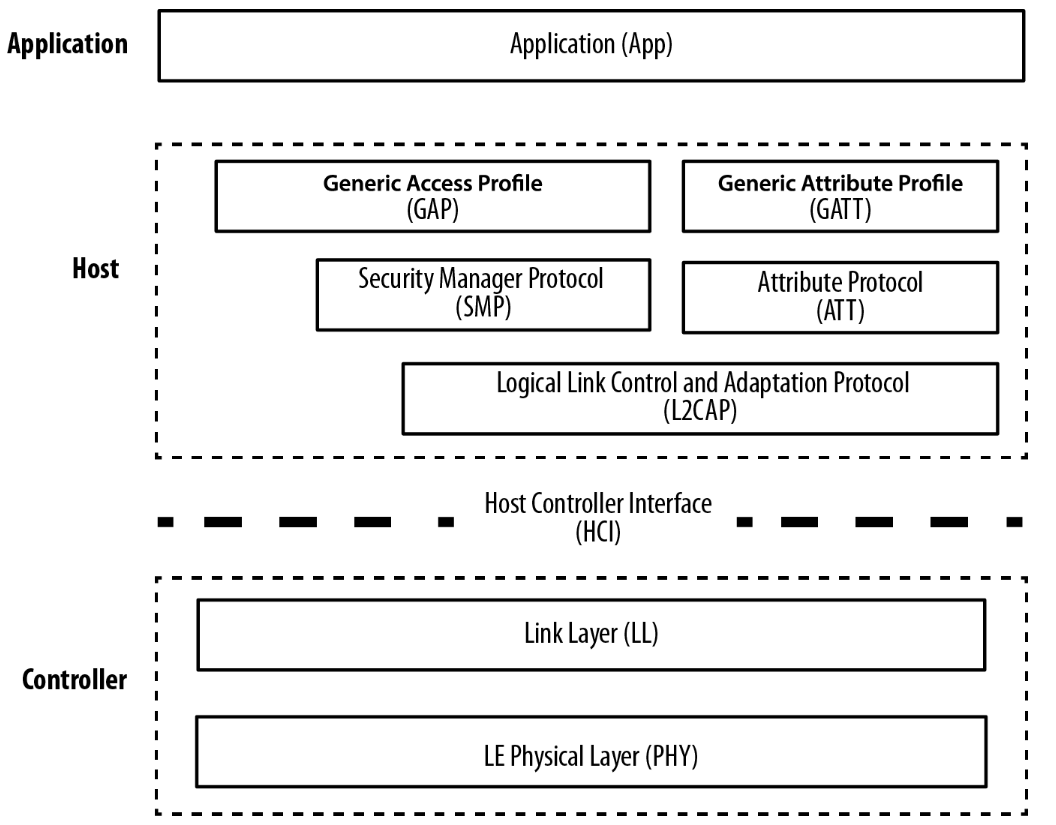
\includegraphics[scale=0.4]{figures/ble_hardware.png} % TODO hacer que esto no quede horrible
    \caption[Estructura hardware de un dispositivo BLE]{Estructura hardware de un dispositivo BLE}
   	\label{figuraBLEHardware}
\end{figure}

\subsection{Controlador}
\label{makereference2.2.1}

\textbf{Capa Física (Physical Layer, PHY).} La capa física es la que contiene los circuitos capaces de comunicarse de forma analógica, modulando y demodulando las señales analógicas y transformándolas en digitales.
Como ya se ha mencionado, la radio usada para BLE utiliza la banda ISM de 2,4 GHz. Esta banda se divide en 40 canales, desde los 2,4000 GHz hasta los 2,4835 GHz. De estos canales, 37 se utilizan para el envío de datos y los 3 restantes como canales de anuncio, para iniciar conexiones y mandar datos de broadcast.

\begin{figure}[h]%t=top, b=bottom, h=here
	\centering
    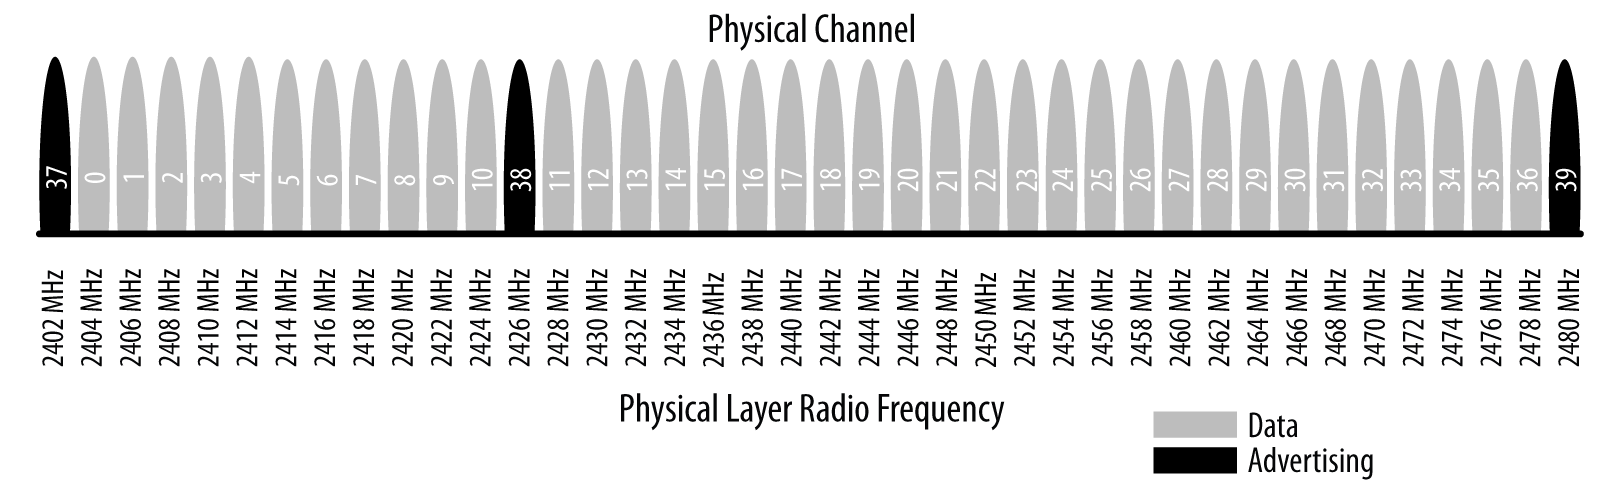
\includegraphics[width=\linewidth]{figures/ble_physical_layer.png} % TODO hacer que esto no quede horrible
    \caption[División de la banda de frecuencia ISM]{División de la banda de frecuencia ISM en 40 canales}
   	\label{figuraBLEPhysicalLayer}
\end{figure}

Para evitar interferencias con otros dispositivos transmitiendo en la misma banda, mayormente WiFi y Bluetooth clásico, el estándar BLE utiliza una técnica llamada \textit{frequency hopping spread spectrum}, que hace que la radio “salte” entre los distintos canales en cada conexión.


\textbf{Capa de Enlace (Link Layer).} Es la parte que actúa de interfaz de la capa física. Normalmente se implementa como una mezcla de software y hardware personalizado. Es responsable de anunciar, escanear, crear y mantener las conexiones. También se encarga de asegurar que los paquetes están correctamente estructurados. Por ello es probablemente la capa más compleja de la arquitectura BLE.


\textbf{Interfaz Anfitrión/Controlador (Host/Controller Interface, HCI).} Muchos dispositivos separan el Anfitrión del Controlador, y para estos casos, el HCI provee una interfaz estandarizada para comunicar los dos dependiendo del método de transporte físico de los datos. Entre estas interfaces se incluyen USB, SDIO o variantes de UART.

\subsection{Anfitrión}
\label{makereference2.2.2}

\textbf{Control Lógico de Enlace y Protocolo de Adaptación (Logical Link Control and Adaptation Protocol, L2CAP).} Esta capa provee dos funcionalidades: actúa como capa multiplexora de los protocolos, es decir, recibe los protocolos de las capas superiores y los encapsula en el formato de paquete estándar BLE (y viceversa). Asimismo, fragmenta los paquetes que se le envían desde las capas superiores para que quepan en los 27 bytes que tienen como máximo los paquetes de transmisión y vuelve a combinar los paquetes fragmentados que recibe.


\textbf{Protocolo de Atributos (Attribute Protocol, ATT).} Define una serie de reglas para acceder a los datos de un dispositivo. Es un protocolo cliente/servidor sin estados, simple, independiente del rol del dispositivo como maestro o esclavo, los dispositivos pueden ser clientes o servidores. Los datos se organizan en forma de atributos, a los que se asigna un handle de 16 bits, un Identificador Único Universal (Universal Unique Identifier, UUID) y una serie de permisos.
ATT define seis tipos de mensajes:
\begin{itemize}
	\item Solicitudes enviadas desde el cliente al servidor.
	\item Respuestas del servidor a una solicitud del cliente.
	\item Comandos enviados del cliente al servidor que no necesitan respuesta. 
	\item Notificaciones enviadas desde el servidor al cliente que no necesitan confirmación.
	\item Indicaciones enviadas desde el servidor al cliente.
	\item Confirmaciones enviadas por el cliente en respuesta a una indicación.
	\item De este modo ambos pueden establecer una comunicación con mensajes que requieran o no respuesta.
\end{itemize}


\textbf{Perfil de Atributo Genérico (Generic Attribute Profile, GATT).} Este perfil se asienta en el Protocolo de Atributos, y define los tipos de atributos y cómo se utilizan. 
Para ello utiliza una jerarquía de capas y un modelo de abstracción de datos. Los datos ahora se encapsulan en servicios, que a su vez consisten en una o más características que pueden estar definidas por un descriptor. Estas capas se sirven de metadatos para dar más información sobre los datos que se están manejando, como nombres, unidades, etc.
Este perfil y el Perfil de Acceso Genérico son importantes a la hora de comunicar dispositivos por BLE, por lo que se explicarán con detalle más adelante.


\textbf{Perfil de Acceso Genérico (Generic Access Profile, GAP).} Define cómo los dispositivos realizan procedimientos de control como el descubrimiento de otros dispositivos, conexiones entre éstos o la seguridad, es decir, dicta cómo interactúan dos dispositivos en un nivel más bajo.
GAP establece diferentes normas y conceptos para regular y estandarizar las operaciones a bajo nivel de los dispositivos:
\begin{itemize}
	\item Roles en los que los dispositivos pueden operar, estableciendo restricciones e imponiendo determinados comportamientos. Se explican con más detalle en las secciones~\ref{makereference2.3.1} y~\ref{makereference2.3.2}.
	\item Modos operacionales, que establecen estados a los que un dispositivo puede cambiar durante un determinado periodo de tiempo para lograr un objetivo, como por ejemplo permitir su descubrimiento o de qué modo permite realizar la conexión.
	\item Procedimientos operacionales para asegurar una comunicación constante mediante una secuencia de acciones.
	\item Aspectos de la seguridad, incluyendo modos y procedimientos.
	\item Formatos de datos adicionales para datos no protocolarios.
\end{itemize}


\textbf{Gestor de Seguridad (Security Manager, SM).} Define los protocolos y sus modos de operar para gestionar la integridad de los enlaces, la autenticación y el cifrado entre dispositivos Bluetooth, y provee las funciones de seguridad que se pueden utilizar para asegurar casi cualquier nivel de seguridad que sea necesario para las diversas aplicaciones.
 
\subsection{Aplicación}
\label{makereference2.2.3}

La aplicación es la capa más alta y la responsable de contener la lógica, la interfaz de usuario y el manejo de los datos de todo lo relacionado con el caso de uso particular que se esté implementando. Es por ello que su arquitectura dependerá en gran medida de la implementación particular. 

\section{Descubrimiento de dispositivos y enlazado}
\label{makereference2.3}

BLE tiene un único formato de paquete que soporta dos tipos: de datos y de anuncio, esto reduce la complejidad de la implementación de la pila de protocolos.

Los paquetes de anuncio tienen como propósito retransmitir datos sin necesidad de una conexión o descubrir esclavos para iniciar una conexión.  Tienen una capacidad útil de 31 bytes, que se utilizan para incluir información sobre el dispositivo y sus capacidades, pero también se pueden incluir los datos que se quieran transmitir. Estos paquetes se envían a intervalos definidos previamente, que pueden ir desde los 20 ms hasta los 10.24 s. Con un intervalo más corto se aumenta la frecuencia de envío de información, pero también significa que tiene un mayor consumo. En nuestro caso definimos un intervalo de 1 s.

Como explicamos anteriormente, BLE utiliza como máximo tres canales de frecuencia para mandar los paquetes de anuncio, y debido a que el dispositivo que anuncia y el que escanea no están sincronizados de ningún modo, los paquetes se recibirán cuando ambos se solapen aleatoriamente, como se ve en el ejemplo presentado en la Figura~\ref{figuraBLEScan}.

\begin{figure}[h]%t=top, b=bottom, h=here
	\centering
    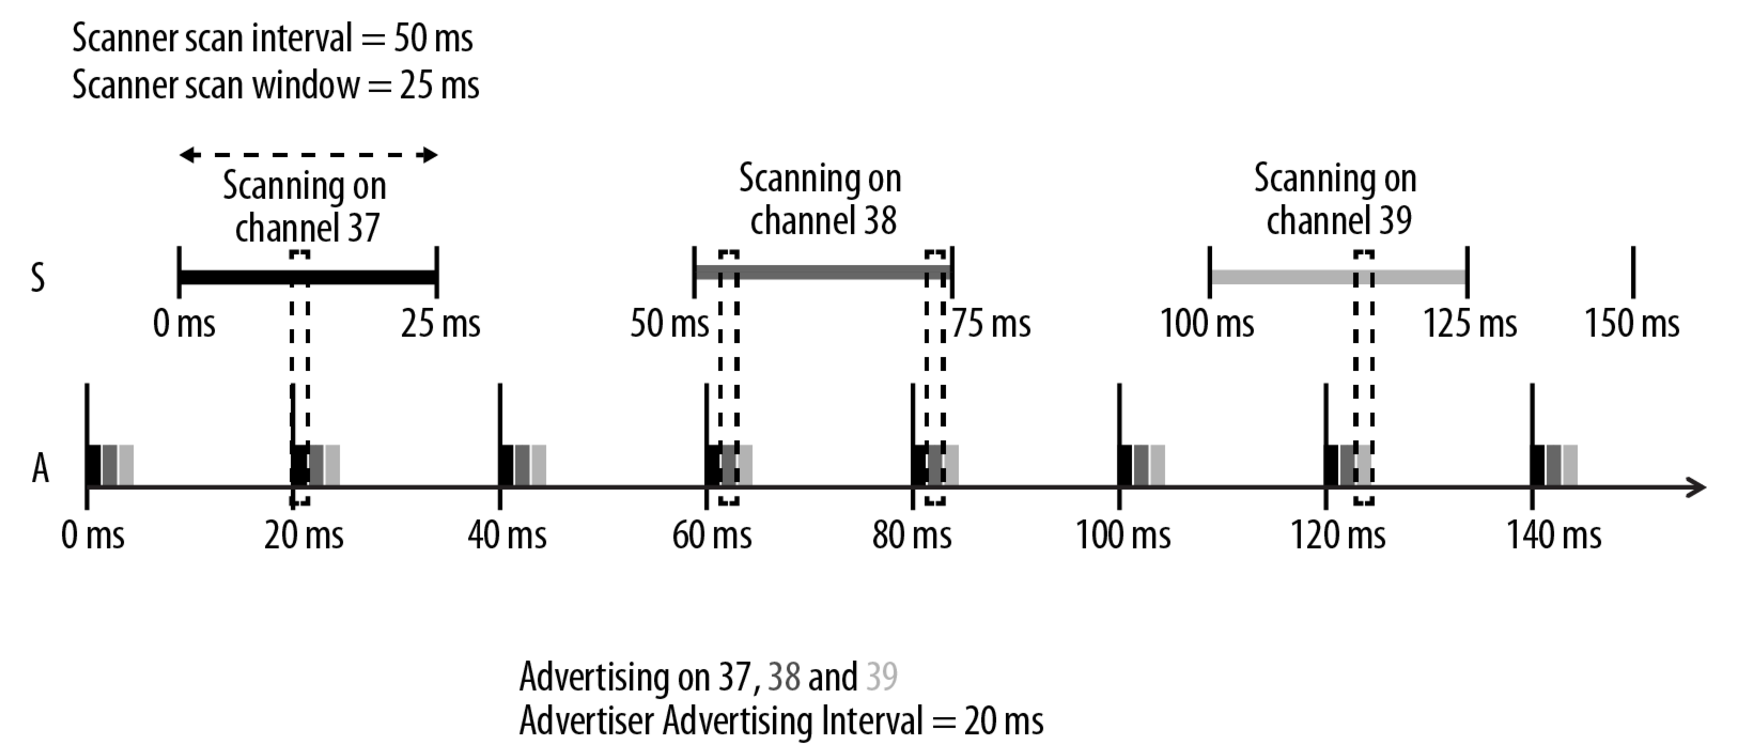
\includegraphics[width=\linewidth]{figures/ble_scan_example.png} % TODO hacer que esto no quede horrible
    \caption[Ejemplo de escaneo BLE]{Ejemplo de escaneo en BLE.}
   	\label{figuraBLEScan}
\end{figure}

Un dispositivo BLE puede comunicarse con el mundo exterior mediante dos vías: \textbf{broadcasting} y \textbf{conexiones}.

\subsection{Modo Broadcast}
\label{makereference2.3.1}

Mediante broadcasting es posible enviar datos en un único sentido a cualquier dispositivo que esté escaneando en el radio de escucha. Es la única forma de mandar datos a más de un dispositivo a la vez.
 
Los dispositivos pueden tomar los siguientes roles GAP:
\begin{itemize}
	\item Broadcaster: envía periódicamente paquetes, sin importar si hay otros dispositivos escuchando.
	\item Observador: escanea las frecuencias establecidas para recibir estos paquetes. 
\end{itemize}

Como se ha explicado antes, el método utilizado para mandar información mediante broadcasting es el de los paquetes de anuncio. BLE permite enviar un segundo paquete por si se necesita mandar más información. Este método, llamado Scan Response, consiste en que el observador que encuentra la señal del broadcaster manda una petición para recibir el segundo paquete. Este segundo paquete de anuncio dispone de otros 31 bytes, haciendo un total de 62 bytes.

\begin{figure}[h]%t=top, b=bottom, h=here
	\centering
    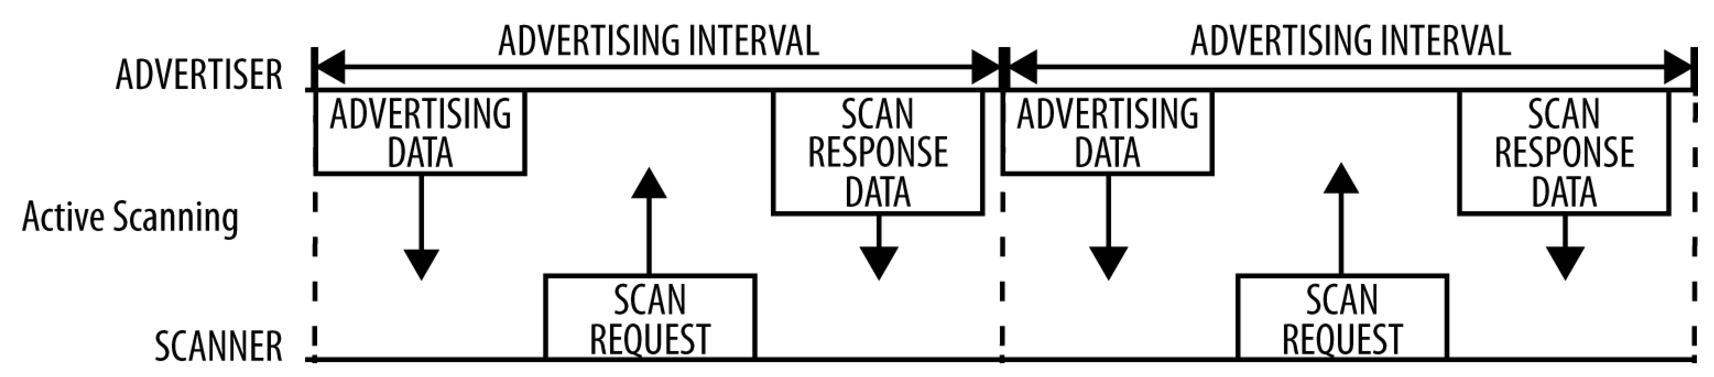
\includegraphics[width=\linewidth]{figures/ble_scan_response.png} % TODO hacer que esto no quede horrible
    \caption[Esquema de Scan Response]{Esquema de Scan Response. El dispositivo que escanea recibe un paquete de advertising y envía esta respuesta para requerir un segundo paquete con más información.}
   	\label{figuraBLEScanResponse}
\end{figure}

Si se desea que la comunicación se realice en los dos sentidos, o una mayor privacidad (dado que, en modo broadcast, todos los dispositivos que escuchan reciben la misma información), o bien se necesita enviar más datos de los que es posible con el modo broadcast, tendremos que usar el modo conexión.

\subsection{Modo Conexión}
\label{makereference2.3.2}

Una conexión permite un intercambio de paquetes de forma periódica y permanente entre dos dispositivos. En este modo tenemos dos roles GAP:

\begin{itemize}
	\item Central (maestro): escanea las frecuencias predefinidas en busca paquetes de advertising y es el encargado de realizar las conexiones. Una vez conectado, es el encargado de gestionar la sincronización y de iniciar el envío periódico de datos. Dado que los requisitos computacionales del rol de maestro son mayores que los de los esclavos, este rol suele recaer en los dispositivos con una CPU y memoria más avanzados, como un smartphone o una tablet.

	\item Periférico (esclavo): se encarga de enviar los paquetes de advertising para que los centrales puedan encontrarlos y de aceptar las conexiones entrantes. El protocolo BLE está optimizado para requerir pocos recursos, en términos de energía y memoria, para la implementación de este rol.
\end{itemize}

La principal ventaja de las conexiones es la posibilidad de organizar los datos que se envían mediante el uso de protocolos para cada campo, más específicamente el Generic Attibute Profile (GATT), que organiza los datos dentro de servicios y características.

\section{Generic Attribute Profile (GATT)}
\label{makereference2.4}

El Perfil de Atributo Genérico expande el Protocolo de Atributo (ATT) estableciendo en detalle cómo intercambiar todos los datos del usuario a través de una conexión BLE. También provee un \textit{framework} para todos los perfiles basados en GATT, que cubren casos de uso específicos y asegura el intercambio entre dispositivos de diferentes marcas. Todos los perfiles BLE estándar están basados en GATT y deben cumplir sus especificaciones para operar correctamente.

\subsection{Jerarquía de datos}
\label{makereference2.4.1}

ATT define el protocolo de atributos, cómo se estructuran y se pueden usar para intercambiar información sobre dispositivos, pero no ofrece más estructura. GATT va más allá y establece una jerarquía de datos estricta para organizar los atributos y permitir su reutilización, de modo que el acceso de información entre cliente y servidor siga una serie de reglas que se puedan usar en cualquier perfil basado en GATT.

\begin{figure}[h]%t=top, b=bottom, h=here
	\centering
    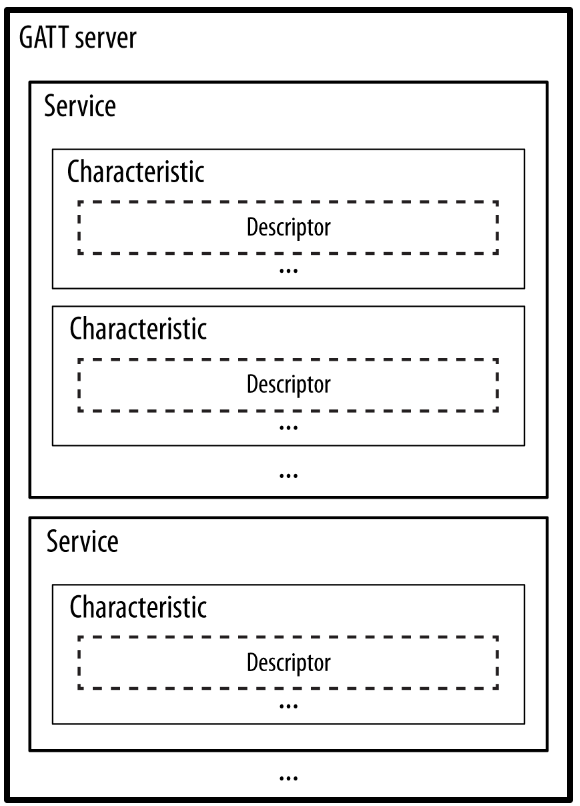
\includegraphics[scale=0.5]{figures/ble_gatt_hierarchy.png} % TODO hacer que esto no quede horrible
    \caption[Esquema de la estructura de datos de GATT]{Esquema de la estructura de datos de GATT}
   	\label{figuraBLEGATTHierarchy}
\end{figure}

Un perfil basado en GATT tendrá entonces, como se muestra en la Figura~\ref{figuraBLEGATTHierarchy}, como mínimo un servicio, con una o más características que encapsulan a los atributos, y que pueden añadir más información a través de un descriptor.

\textbf{Atributo.} Los atributos son las entidades de datos más pequeñas definidas en GATT y ATT. Son piezas de información direccionables que pueden contener los datos del usuario o metadatos sobre la estructura y el agrupamiento de los diferentes atributos contenidos en el servidor.

Dado que GATT y ATT sólo pueden operar con atributos, los clientes y servidores que deseen realizar una interacción deberán organizarse de esta forma. Cada atributo contiene los datos del usuario e información sobre el propio atributo, contenidos en los siguientes campos:
\begin{itemize}
	\item \textit{Handle.} Es la parte que hace a un atributo direccionable. Consiste en un identificador de 16 bits para cada atributo en un servicio GATT particular, y se garantiza que no se modificará entre transacciones o conexiones.  El valor 0x0000 denota un handle inválido, por lo que el rango de handles disponible es de 0xFFFF (65535), aunque en la práctica el número de atributos en un servidor es más cercano a la docena.

	\item \textit{Tipo.} Esta parte consiste en un UUID de 16, 32 o 128 bits que determina qué tipo de datos están presentes en el campo de valor del atributo, permitiendo por ejemplo mecanismos para encontrar un atributo directamente por su tipo.

	\item \textit{Permisos.} Los permisos son metadatos que especifican qué operaciones se pueden ejecutar en cada atributo y con qué requisitos de seguridad. ATT y GATT definen los siguientes permisos:
	\begin{itemize}
		\item Permisos de acceso: similares a los permisos presentes en un archivo.  Define si se puede acceder a un valor como sólo de lectura, de escritura, de ambos o de ninguno.
		\item Encriptación: determina si es necesario algún nivel de encriptación para acceder al valor. Puede no necesitarla, o exigir una encriptación con o sin autenticación.
		\item Autorización: determina si se necesita o no permiso del usuario para acceder al atributo.
	\end{itemize}

	\item \textit{Valor.} Contiene los propios datos sin restricción de qué tipo sean, aunque con un máximo de 512 bytes según la especificación. Dependiendo del tipo de atributo, puede contener información adicional sobre el atributo o un valor útil.
\end{itemize}

\textbf{Servicio.} Los servicios agrupan atributos conceptualmente relacionados. La forma de definir un servicio es a través de uno o más atributos denominados definición de servicio, de los cuales el primero es el que actúa de declaración de servicio y el resto pueden definir las siguientes capas, como características y descriptores.

Se puede comparar un servicio con una clase en cualquier lenguaje de programación orientado a objetos. 

\textbf{Característica.} Las características se pueden entender como contenedores para los datos del usuario. Siempre incluyen dos atributos: la declaración de la característica, que ofrece metadatos sobre los datos en sí, y el valor de la característica, que es un atributo completo con los datos del usuario. Adicionalmente, una característica puede contener un descriptor, que es un atributo que provee de más metadatos.

\textbf{Descriptor.} Se utilizan principalmente para proveer al cliente con información adicional sobre las características y su valor. Se ubican siempre entre la definición de la característica y el valor del atributo de la característica y están compuestos por un único atributo cuyo UUID define el tipo de descriptor y el campo de valor contiene lo que esté definido para ese tipo de descriptor.

A continuación se detallan algunos de los descriptores más utilizados:

\begin{itemize}
	\item \textit{Descriptor de usuario de una característica:} contiene una descripción que el usuario puede leer consistente en una cadena de caracteres en UTF-8. Por ejemplo “Temperatura en el salón”.
	\item \textit{Descriptor de configuración de la característica por el cliente:} actúa como un “interruptor”, deshabilitando las actualizaciones que envía el servidor.
	\item \textit{Descriptor de formato de presentación de una característica:} contiene el tipo de variable de la característica, por ejemplo booleano, cadena de caracteres, enteros, etc.
\end{itemize}

\subsection{Roles}
\label{makereference2.4.2}

GATT define dos roles que pueden adoptar los dispositivos interconectados, que hereda directamente del Protocolo de Atributos (ATT):
\begin{itemize}
	\item \textbf{Cliente.} Envía peticiones al servidor y recibe respuestas. El cliente GATT no tiene conocimiento sobre los atributos del servidor por adelantado, por lo que primero tiene que recopilar información sobre éstos mediante un descubrimiento de servicios.

	\item \textbf{Servidor.} Recibe las peticiones del cliente y responde en consecuencia. Es el rol responsable de guardar los datos y de hacer que estén disponibles para el cliente, organizándolos en atributos. Todos los dispositivos BLE que se vendan deben incluir al menos un servidor GATT básico, aunque únicamente envíe un error como respuesta.
\end{itemize}

\subsection{UUIDs}
\label{makereference2.4.3}

Un \textit{Identificador Único Universal} (UUID) es un número de 128 bits (16 bytes) que garantiza (al menos con una gran probabilidad) que es único globalmente. UUID es usado en otros protocolos aparte de Bluetooth, y su formato, uso y generación se especifican en el ISO/IEC 9834-8:2005.

Dado que 16 bytes ocuparía gran parte del tamaño disponible en los 27 bytes de los paquetes de datos, la especificación BLE añade dos formatos adicionales: UUIDs de 16 o 32 bits, y se forman definiendo un “final” del UUID que es constante en todos los dispositivos BLE, en los que se sustituyen los 32 primeros bits:

\begin{center}xxxxxxxx-0000-1000-8000-00805F9B34FB\end{center}

donde xxxxxxxx son los bits a sustituir.


%In this chapter, I want to refer to Chapter~\ref{makereference},
%so I'm going to use the slash ref command along with the
%"makereference" label which I assigned back at the beginning of
%Chapter 1.

%\section{Page Number References}
%\label{makereference2.1} I should also be able to refer to a
%specific page number, such as page~\pageref{makereference}.  Of
%course, I'll need to have a slash label command and a unique name
%in each section that I want to be able to refer to later in the
%text.

%\section{Referring to Sections Within Chapter 1}
%\label{makereference2.2} Now, I'm going to refer to different
%sections within Chapter 1. I gave an example of a figure in
%section~\ref{makereference1.1} and an example of a table in
%section~\ref{makereference1.2}.  In
%section~\ref{makereference1.3}, we looked at examples of
%bibliographic citations.
